Databasen er lavet i sqlite.  Formålet med databasen er todelt,
opbevaring af metadata og opsamling af statestik fra kørsler.
Problemet med dette er at når databasen skal konstrueres, er det ikke
muligt at sige noget definitivt omkring statestik delen af databasen.
At splitte databasen op i to, er en mulighed.  En del af de udvidede
løsninger opridset i synopsisen benytter en del af metadataerne omkring
billederne, derfor er denne løsning af tvivlsom anvendlighed.  En
løsning, der tilbyder udvidelse, må derfor være at tilstræbe.
Basisløsningen består udelukkende af opbevaringen af metadata, grunden
til dette er udelukkende planlægning af projektet.  Database skemaet
til basisløsningen bygger endnu videre på den struktur, der er
udleveret af \cite{wgahu}.

\begin{center}
\begin{tabular}{|l||c|c|c|c|c|c|}
    \hline
    \bf{artist} \hspace{0.5cm} & \underline{artistId} & name & born & died & school & timeline \\\hline
\end{tabular}

\begin{tabular}{|l||c|c|c|c|c|c}
    \hline
    \bf{painting} \hspace{0.5cm} & \underline{paintingId} & artistId & title & date & paint & $\cdots$ \\\hline
\end{tabular}\\ \vspace{0.2cm}\hspace{1.2cm}
\begin{tabular}{c|c|c|c|c|c|c}
    \hline
    $\cdots$ & material & location & url & form & type & $\cdots$ \\\hline
\end{tabular}\\ \vspace{0.2cm}\hspace{1.4cm}
\begin{tabular}{c|c|c|c|c|c|}
    \hline
    $\cdots$ & realHeight & realWidth & height & width & filepath \\\hline
\end{tabular}

\begin{tabular}{|l||c|c|c|c|c|c|c|}
    \hline
    \bf{run} \hspace{0.5cm} & \underline{runId} & trsh1 & trsh2 & lo & up & marginPercentage & method \\\hline
\end{tabular}

\begin{tabular}{|l||c|c|c|c|c|c|}
    \hline
    \bf{result} \hspace{0.5cm} & \underline{resultId} & runId & paintingId & cutRatio & cutNo & numberOfRegions \\\hline
\end{tabular}

\begin{tabular}{|l||c|c|c|c|c|c|c|}
    \hline
    \bf{region} \hspace{0.5cm} & \underline{regionId} & resultId & x & y & height & width & area \\\hline
\end{tabular}
\end{center}

\newpage
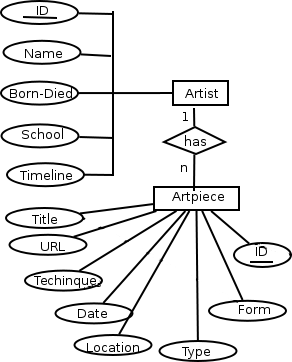
\includegraphics[scale=0.9]{afsnit/vores_implementation/billeder/ER}

% vim: set tw=72 spell spelllang=da:
